\section{Backtesting framework and methodology}
\label{sec:framework}
\subsection{Rolling estimates and execution}
The framework separates models, strategies and portfolio accounting. Models convert the available return history into estimates; strategies use those estimates to choose target weights; the simulator tracks positions, trades, fees and value. Several strategies can share the same model estimates while maintaining independent portfolios.

Every five trading days we fit PCA to the latest 500 returns, standardizing each stock within that window and retaining five components. The factor regression uses the active PCA weights throughout its own window and refits whenever the PCA basis changes. Treynor--Black estimates alphas over 250 days and refits daily. Snapback uses a 100-day regression and a factor model fitted through the previous day, so the return being judged does not enter the fit that judges it.

Positions carried into day $t$ earn that day's return before the next adjustment. Weights chosen at the close of $t$ therefore earn
\[
r_{\mathrm{port},t+1}^{\mathrm{gross}}=\sum_i w_{i,t}r_{i,t+1}.
\]
The baseline assumes fills at the signal's close and deducts 5 basis points per dollar bought or sold. Turnover is measured from drifted positions to the new targets. Portfolios hold cash during warm-up; cash earns zero interest. A one-day execution delay tests dependence on immediate fills. Truncating the original backtest at December 2011 leaves earlier positions unchanged up to rounding of order $10^{-13}$.

\begin{figure}[htbp]
    \centering
    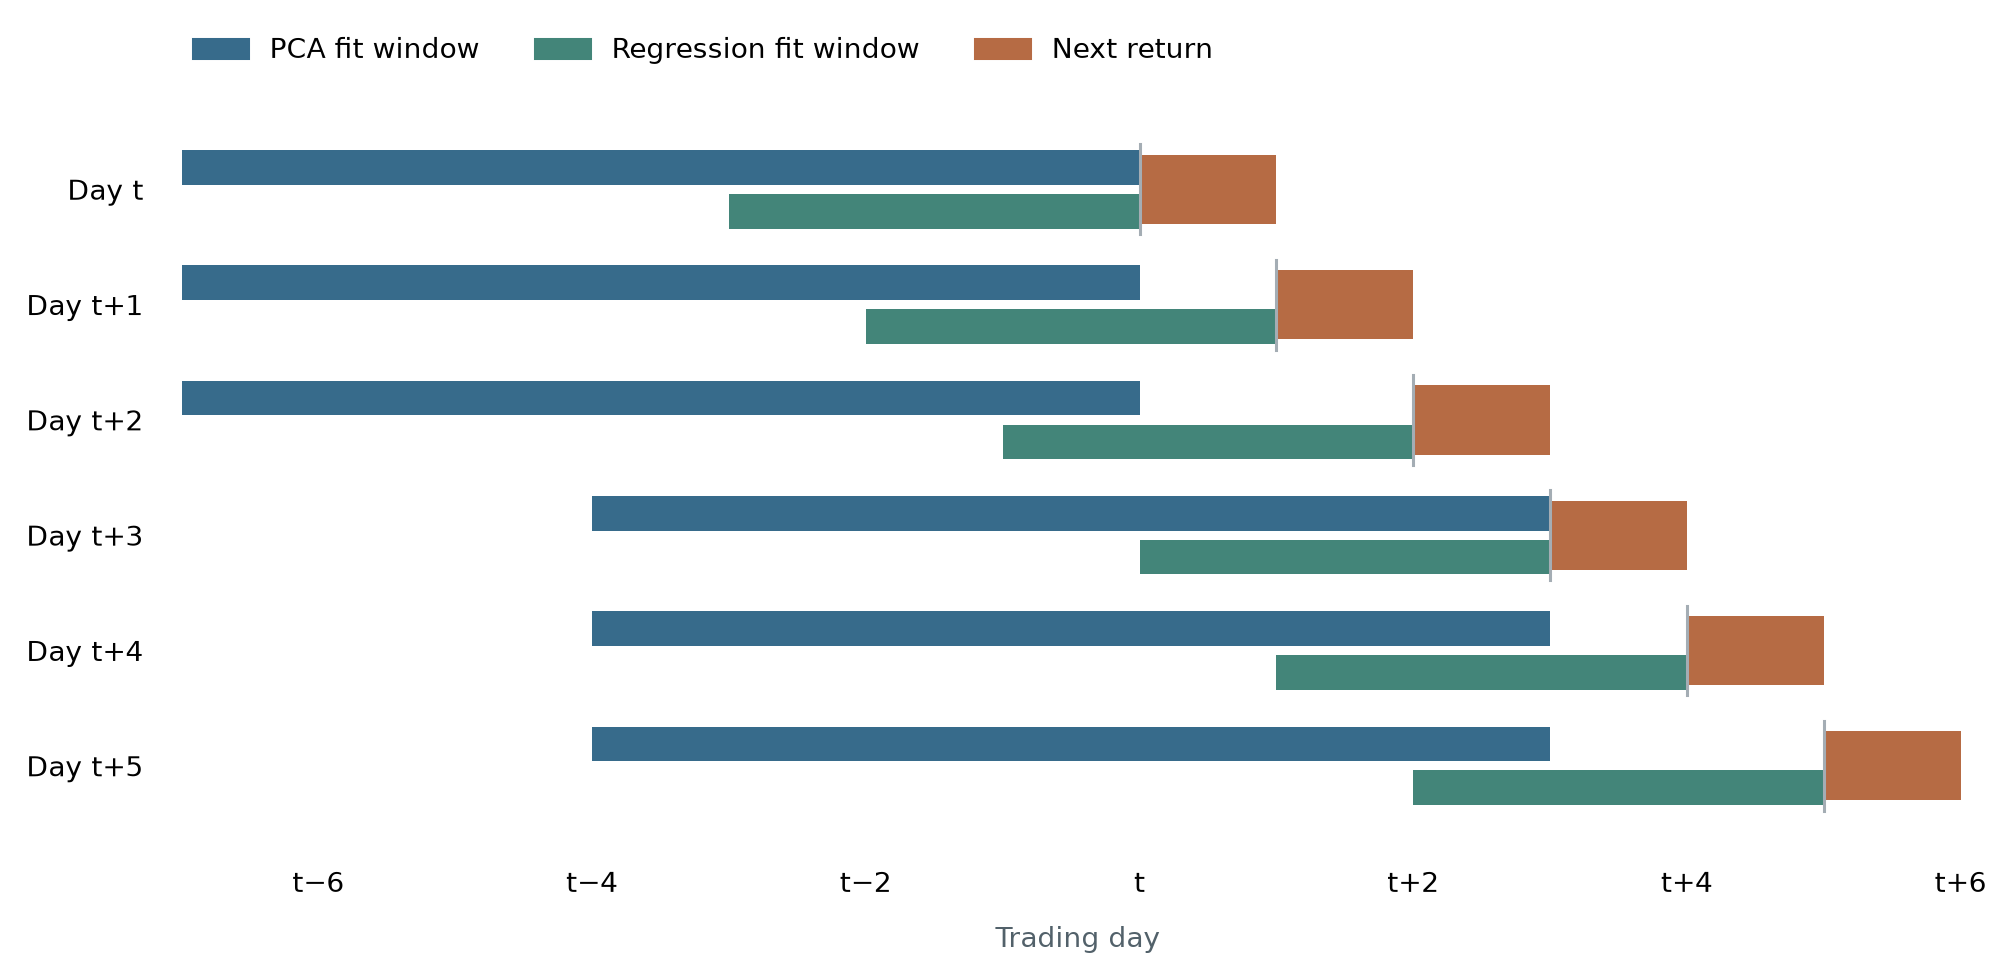
\includegraphics[width=0.85\linewidth]{figures/framework_walkforward.png}
    \caption{Walk-forward estimation over six consecutive decision dates.
    Each row represents the portfolio decision at the indicated day's
    close, marked by the vertical gray line. Blue bars identify the
    observations used by the active PCA estimate, and green bars identify
    the regression window. In this example, PCA refits at \(t\) and
    \(t+3\), so its estimation window remains unchanged for three rows
    before advancing. The regression refits daily using the active PCA
    weights, including a new factor basis when PCA updates. Orange bars
    show the subsequent return interval earned by the chosen portfolio.
    Estimation periods lie entirely before or at the decision close,
    while portfolio returns occur afterward. Window lengths and the
    three-day PCA interval are illustrative rather than strategy defaults.}
    \label{fig:framework-walkforward}
\end{figure}

\subsection{Evaluation and limitations}
We compare gross and net returns, annual performance, drawdowns, turnover, parameter sensitivity, calibration and the 2018--2023 historical holdout. Parameters selected using the earlier period are evaluated on later observations while model estimates continue to update. Parameter comparisons use common start dates after the longest warm-up. This preserves information timing but does not remove the effects of repeated strategy development.

Sharpe ratios use daily returns, a zero risk-free rate and annualization by $\sqrt{252}$. For the assignment's information ratio, we subtract fitted market exposure from portfolio returns and annualize the mean divided by the standard deviation of the remainder. Strategy market betas use the equal-weighted stock universe; Question 4 instead uses the value-weighted U.S. market benchmark.

The original universe's selection procedure is unverified and may omit failed firms and later entrants. Closing-price fills, proportional fees, and the omission of impact and stock-specific borrow costs can overstate implementable returns. Repeated testing can also overfit historical periods. These limits remain relevant even when estimates use only past data. Appendix~\ref{app:framework} gives the implementation, walk-forward diagrams, numerical benchmarks and fuller discussion.
